\documentclass[a4paper,12pt]{article}
\usepackage[utf8]{inputenc}
\usepackage[T1]{fontenc}

\usepackage[left=1.5cm, right=1.5cm, top=2cm, bottom=2cm, twoside]{geometry}

\usepackage{esvect}
\usepackage{siunitx}
\usepackage{fancybox}

\usepackage{amsmath}
\usepackage{amsfonts}
\usepackage{amssymb}
\usepackage{amsthm}

\usepackage{braket}
\usepackage{graphicx}
\usepackage{mathptmx}
%\usepackage{tikz}
\usepackage{pgfplots}
\usepackage{siunitx}
\usepackage{hyperref}


\usepackage{pstricks}
\usepackage{pstricks-add}
\usepackage{pst-plot}
\pgfplotsset{compat=1.17}

\usepackage[french]{babel}
%Raccourcis de la flemme
\newcommand{\R}{\mathbb{R}}
%\newcommand{\C}{\mathbb{C}}
\newcommand{\D}{\, \mbox{d}}

\hypersetup{
 pdfauthor={Tanneguy Blandin},
 pdftitle={Devoir maison: Physique du solide},
 pdfkeywords={},
 pdfsubject={},
 pdfcreator={Me}, 
 pdflang={French}}

%Définition des numéros d'éxercices
\newcounter{numExo}
\newcounter{partExo}
\newcounter{numQuestion}
\newcounter{numSubQuestion}


\newcommand{\exercice}[1]{%
  \stepcounter{numExo}%
  \setcounter{partExo}{0}%
  \setcounter{numQuestion}{0}%
  \setcounter{numSubQuestion}{0}%
    \noindent
    \section*{Exercice \arabic{numExo}: #1}
    \addcontentsline{toc}{section}{\protect\numberline{}Exercice \arabic{numExo}: #1}
}
\newcommand{\partexo}[1]{%
  \stepcounter{partExo}%
    \setcounter{numQuestion}{0}%
    \setcounter{numSubQuestion}{0}%
    \noindent
    \subsection*{\Alph{partExo} -- #1}
    \addcontentsline{toc}{subsection}{\protect\numberline{}\Alph{partExo}: #1}
    }

\newcommand{\Question}{%
  \stepcounter{numQuestion}%
  \setcounter{numSubQuestion}{0}%
 \par\noindent \textbf{\arabic{numQuestion}.\hspace{2pt}}}


\newenvironment{question}%
{%
\ttfamily %
  \stepcounter{numQuestion}%
  \setcounter{numSubQuestion}{0}%
 \par\noindent \textbf{\arabic{numQuestion}}
}%
{%
\normalfont
}

\newenvironment{info}%
{%
\ttfamily %
}%
{%
\normalfont
}

\newcommand{\subquestion}{%
  \stepcounter{numSubQuestion}%
  \par{}\hspace{3pt}\textbf{\arabic{numSubQuestion}.\hspace{2pt}}}


%%INFO DOC
\title{Devoir maison \\ Physique des matériaux \\ \large{\textsc{insa} Rennes -- 3 SGM}}
\date{Mars 2021}
\author{Tanneguy Blandin}

  
\begin{document}
\maketitle


\exercice{Cristal bidimensionnel}

\partexo{Réseau}

\begin{figure}[htb]
  \centering
  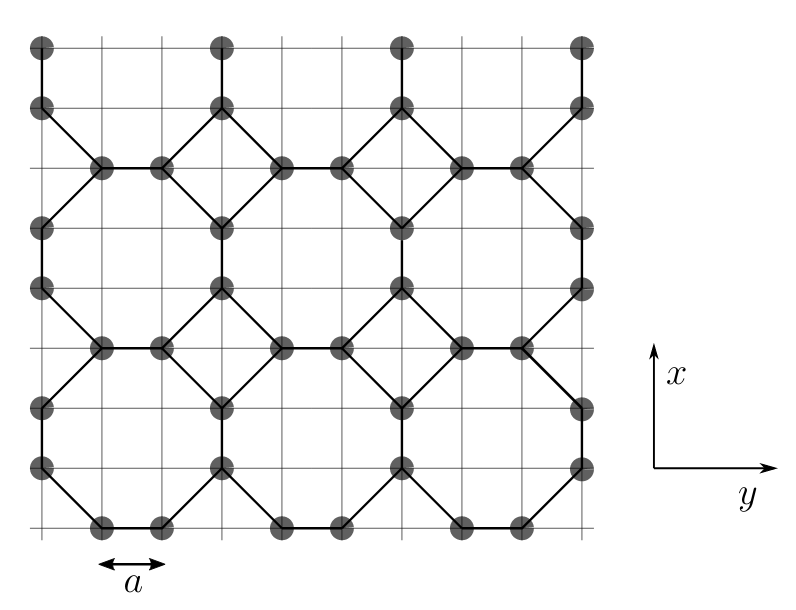
\includegraphics[width=0.5\textwidth]{./pictures/cristal2D.png}
  \caption{Cristal 2D}
  \label{fig:cristal2D}
\end{figure}

\begin{question}
  Donner les coordonnées des vecteurs $(\vv{a},\vv{b})$ qui définissent une maille primitive de ce réseau dans le repère $Oxy$ orthonormé, en fonction de $a_0$.
\end{question}

La maille est une maille carrée, les vecteurs de la maille élémentaire de ce réseau sont $\vv{a}=(3a_0,0)$ et $\vv{b}=(0,3a_0)$. Cependant, la maille primitive
ne doit être consitué aue d'un unique noeud du réseau. AHHH

\begin{question}
  Préciser la nature du réseau direct et son paramètre de maille $a$
\end{question}



\begin{question}
  Préciser le motif associé à ce cristal : nombre d'atomes et position en fonction des vecteurs $\vv{a}$ et $\vv{b}$
\end{question}


\begin{question}
  Calculer l'aire de la maille unitaire, en fonction de $a_0$
\end{question}

\begin{question}
  Calculer le nombre d'atomes par unité de surface. Application numérique en \si{\squared\meter}.
  \end{question}

\begin{question}
  Exprimer les coordonnées des vecteurs du réseau réciproque $(\vv{a*}, \vv{b*})$, en fonction de $a_0$ dans le repère $Oxy$
\end{question}


\begin{question}
  Dessiner le réseau réciproque et le première zone de Brillouin
\end{question}
\begin{question}
  Dans la première zone de Brillouin, placer les points $\Gamma$ ,$X$ de coordonnées $(\pi/a,0)$ et $M$ de coordonnées $(\pi/a,\pi/a)$.
  \end{question}




\partexo{Bandes d'énergie}
\begin{info}
  On suppose que l'énergie des électrons de conduction est représentée par :
  \begin{equation}\label{equ:enerelectron}
    E_c(\vv{k})= \alpha  - 2 \gamma \left( \cos(k_x a)  + \cos(k_y a)    \right)
  \end{equation}
\end{info}


\Question En prenant l'équation~\ref{equ:enerelectron} pour définir l'énergie des électrons de conduction, nous pouvons calculer l'énergie aux points caractéristiques de la maille en prenant $\alpha = \SI{2,5}{\eV}$ et $\gamma = \SI{0,5}{\eV}$:
\begin{itemize}
\item En $\Gamma$ ($\vv{k}=(0,0)$), nous avons: $E_{c\Gamma} = \alpha - 4\gamma= \SI{0,5}{\eV}$.
\item En $X$ ($\vv{k}=(\pi/a,0)$), nous avons: $E_{cX} = \alpha = \SI{2,5}{\eV}$ .
\item En $M$ ($\vv{k}= (\pi/a,\pi/a)$), nous avons: $E_{cM} = \alpha + 4\gamma = \SI{4,5}{\eV}$.
\end{itemize}

\Question En déterminant la ou les composantes de $\vv{k}$ qui varie ou varient en fonction de la direction dans laquelle nous nous déplaçons dans le cristal, nous pouvons réécire la fonction $\vv{k}$ pour chaque direction:
\begin{itemize}
\item Sur la direction $\Gamma X$ ou $\Delta$, nous pouvons définir $\vv{k}$ en fonction de $x$ de la manière suivante:
  \begin{align*}
    [0,\frac{\pi}{a}] & \rightarrow [0,\frac{\pi}{a}]^2\\
    x                 & \mapsto    \vv{k} = (x,0) \\
  \end{align*}
  Nous pouvons donc définir la variation de l'énergie dans cette direction:
  \begin{equation}\label{equ:Delta}
    x\in[0,\frac{pi}{a}] \quad E_{c\Delta} = \alpha - 2\gamma\left(1+\cos(ax)\right)
  \end{equation}

\item Sur la direction $\Gamma M$, nous pouvons définir $\vv{k}$ en fonction de $x$x de la manière suivante:
  \begin{align*}
    [0,\frac{\pi}{a}] & \rightarrow [0,\frac{\pi}{a}]^2\\
    x                 & \mapsto    \vv{k} = (x,x) \\
  \end{align*}
  Nous pouvons donc définir la variation de l'énergie dans cette direction:
  \begin{equation}\label{equ:GammaX}
    x\in[0,\frac{pi}{a}] \quad E_{c\ \Gamma X} = \alpha - 4\gamma\cos(ax)
  \end{equation}

\item Sur la direction $XM$, nous pouvons aussi définir $\vv{k}$ en fonction de $x$:
  \begin{align*}
    [0,\frac{\pi}{a}] & \rightarrow [0,\frac{\pi}{a}]^2\\
    x                 & \mapsto    \vv{k} = (\frac{\pi}{a},x) \\
  \end{align*}
  Nous pouvons donc définir la variation de l'énergie dans cette direction:
  \begin{equation}\label{equ:XM}
    x\in[0,\frac{pi}{a}] \quad E_{c\ XM} = \alpha - 2\gamma(\cos(ax)-1)
  \end{equation}
\end{itemize}


Nous pouvons représenter l'évaluation de l'énergie en fonction de la position sur les principales directions, c'est que que nous faisons sur la figure

\begin{figure}[htb]
  \centering
  \begin{pspicture}(-4,-1)(7.14,5)
    \psline[showpoints=true, dotstyle=pentagon*](-3.14159,0)(0,0)(3.14159,0)(6.283185,0)
    \psline[showpoints=true, dotstyle=pentagon*]{->}(0,0)(0,1)(0,2)(0,3)(0,4)(0,5)
    %% M->Gamma
    \def\EMG{x RadtoDeg cos -2 mul 2.5 add}
    \psplot{-3.141592}{0}{\EMG}
    \uput[d](-3,0){$M$}
    %% Gamma -> X
    \def\Delta{x RadtoDeg cos 1.5 sub neg}
    \psplot{0}{3.141519}{\Delta}
    \uput[d](0,0){$\Gamma$}
    %% X -> M
    \def\EXM{x 3.141519 sub RadtoDeg cos -1 mul 3.5 add}
    \psplot{3.141519}{6.28318}{\EXM}
    \uput[d](3.141592,0){$X$}
    \uput[d](6.28318,0){$M$}
  \end{pspicture}

\end{figure}



\end{document}

% LocalWords:  Hermitiques Schrödinger Hermitique
